\documentclass[10pt,a4paper]{article}
\usepackage[utf8]{inputenc}
\usepackage[a4paper, margin=1.25cm, top=1.30cm, bottom=1.30cm]{geometry}
\usepackage{amsmath,amssymb}
\usepackage{xcolor}
\usepackage[most]{tcolorbox}
\usepackage{booktabs}
\usepackage{colortbl}
\usepackage{fancyhdr}
\usepackage{graphicx}
\usepackage{enumitem}
\usepackage{needspace}
\usepackage{array}
\usepackage{hyperref}

% Exact colors from DL lecture notes
\definecolor{themeblue}{rgb}{0.1686, 0.3529, 0.5294}   % #2B5A87
\definecolor{lightbg}{rgb}{0.9098, 0.9333, 0.9569}     % #E8EEF4
\definecolor{accentred}{rgb}{0.7843, 0.2706, 0.2275}   % #C8453A
\definecolor{accentgreen}{rgb}{0.1804, 0.4902, 0.1961} % #2E7D32
\definecolor{codebg}{rgb}{0.96, 0.97, 0.98}

% Header and Footer
\pagestyle{fancy}
\fancyhf{}
\fancyhead[L]{\textcolor{themeblue}{\small Midterm Revision Summary --- Wireless Communications \& Networks}}
\fancyhead[R]{\textcolor{themeblue}{\small WCNS (Fourth Year, S7)}}
\renewcommand{\headrulewidth}{0.5pt}
\renewcommand{\headrule}{\hbox to\headwidth{\color{themeblue}\leaders\hrule height \headrulewidth\hfill}}
\fancyfoot[C]{\thepage}

\begin{document}

% Title Block
\begin{center}
    {\LARGE\bfseries\color{themeblue} Wireless Communications \& Networking Systems (WCNS)}\\[2pt]
    {\large\bfseries\color{themeblue} Comprehensive Midterm Revision \& Formula Sheet}\\[2pt]
    {\small\itshape Based on Lectures CH01--CH05, Labs 01--04 \& Past Midterm Exams (ENSIA 2025--2026)}\\[2pt]
    \textcolor{themeblue}{\rule{\textwidth}{0.6pt}}
\end{center}

\vspace{-8pt}

% Scope Box
\begin{tcolorbox}[
    colframe=themeblue,
    colback=lightbg,
    coltitle=white,
    fonttitle=\bfseries\sffamily\small,
    title={Executive Exam Roadmap: High-Yield Topics \& Midterm Structure},
    arc=1.4mm,
    boxrule=0.6pt,
    left=6pt, right=6pt, top=3pt, bottom=3pt
]
\footnotesize
This summary consolidates the theoretical foundations and lab implementations necessary for the WCNS Midterm:
\begin{itemize}[leftmargin=12pt, itemsep=1pt, topsep=1pt]
    \item \textbf{Part 1: Concept MCQs (8.0 pts, 16 Qs, $-0.25$ penalty):} Spectrum rules, propagation mechanisms, noise physics, fading taxonomy, MIMO, and modulation trades.
    \item \textbf{Part 2: Course Core Questions (4.0 pts):} Shannon capacity scaling, constellation Euclidean distance, link budget \& antennas, and urban vehicular fading characterization.
    \item \textbf{Exercise 1: Signal Spectrum \& Filtering (4.0 pts):} Square wave Fourier series, harmonic frequencies, and moving average filter first-null design ($f_{\text{null}} = f_s / M$).
    \item \textbf{Exercise 2: Line Coding \& Modulation (4.0 pts):} Unipolar/Bipolar NRZ, ASK (OOK) \& BPSK waveform drawing ($f_c T_b$ carrier cycles), SNR in dB, BER calculation, and receiver noise immunity comparison.
\end{itemize}
\end{tcolorbox}

\vspace{-2pt}

% =========================================================================
% MODULE 1: TRANSMISSION FUNDAMENTALS & INFORMATION CAPACITY
% =========================================================================
\noindent{\Large\bfseries\color{themeblue} 1. Transmission Fundamentals, Fourier Spectrum \& Capacity Limits}\par\vspace{2pt}

\begin{tcolorbox}[
    colframe=themeblue,
    colback=white,
    arc=1.2mm,
    boxrule=0.5pt,
    left=5pt, right=5pt, top=2pt, bottom=2pt
]
\footnotesize
\textbf{1. Why Modulate?} Antenna size is proportional to wavelength: $L \approx \frac{\lambda}{4} = \frac{c}{4f}$. Baseband signals (e.g., $3\text{ kHz}$) require antennas $\sim 25\text{ km}$ long. Bandpass modulation shifts baseband data onto high-frequency RF carriers ($f_c \gg f_m$), enabling compact antennas and multi-user frequency division (*CH01, CH03*).

\textbf{2. Digital Data vs. Digital Signal:} Modulating digital data directly into digital baseband voltage pulses (e.g., NRZ) has the massive advantage of \textbf{simplicity and low cost of equipment} compared to analog transceivers (*CH05, Slide 5-3*).

\textbf{3. ISM Frequency Bands:} Industrial, Scientific, and Medical bands (e.g., $2.4\text{ GHz}, 5\text{ GHz}$) are \textbf{unlicensed bands} that anyone can transmit on without purchasing government frequency licenses, provided power and spread-spectrum rules are satisfied (*CH04, Slide 4-13*).
\end{tcolorbox}

\vspace{1pt}

\noindent\textbf{\color{themeblue}Square Wave Fourier Decomposition \& Bandwidth Requirements (Exercise 1 Core)}
\begin{itemize}[leftmargin=12pt, itemsep=1.5pt, topsep=1pt]
    \item \textbf{Fourier Series for Square Wave:} A zero-mean periodic square wave of fundamental frequency $f_0 = 1/T$ consists strictly of an infinite sum of \textbf{odd sinusoidal harmonics}:
    \begin{equation}
        x(t) = \frac{4A}{\pi} \sum_{k=1, 3, 5, \dots}^{\infty} \frac{1}{k} \sin(2\pi k f_0 t) = \frac{4A}{\pi} \left[ \sin(2\pi f_0 t) + \frac{1}{3}\sin(2\pi \cdot 3f_0 t) + \frac{1}{5}\sin(2\pi \cdot 5f_0 t) + \dots \right]
    \end{equation}
    \item \textbf{Harmonic Frequencies:} 
    \begin{itemize}[leftmargin=10pt, itemsep=0.5pt]
        \item Fundamental (1st harmonic): $f_1 = f_0$.
        \item First non-zero harmonic after fundamental (3rd harmonic): $f_3 = 3f_0$.
        \item Second non-zero harmonic (5th harmonic): $f_5 = 5f_0$, etc. Even harmonics ($2f_0, 4f_0$) have zero amplitude.
    \end{itemize}
    \item \textbf{Why Digital Square Signals Require Higher Bandwidth than Sine Waves:} A pure sinusoid concentrates 100\% of its energy in a single spectral line at $f_0$ (bandwidth $\approx 0$). In contrast, a square wave contains instantaneous time-domain step discontinuities. Constructing these steep vertical edges requires an \textbf{infinite sum of high-frequency odd harmonics}. Truncating or filtering these harmonics rounds the edges and causes pulse dispersion (*CH02, Lab 01, Lab 02*).
\end{itemize}

\vspace{1pt}

\begin{tcolorbox}[
    colframe=accentgreen,
    colback=white,
    arc=1.2mm,
    boxrule=0.5pt,
    left=5pt, right=5pt, top=2.5pt, bottom=2.5pt
]
\textbf{Channel Capacity Formulas (Nyquist vs. Shannon) --- Exam Favorite:}
\begin{enumerate}[leftmargin=12pt, itemsep=1pt, topsep=1pt]
    \item \textbf{Nyquist Formula (Noiseless Channel):} Sets the theoretical maximum data rate for a channel with bandwidth $B$ and $M$ signaling levels:
    \[
    C = 2B \log_2(M) \quad [\text{bps}], \qquad \text{Baud / Modulation Rate: } D = \frac{R}{\log_2 M} = \frac{R}{L} \quad [\text{symbols/sec}]
    \]
    \item \textbf{Shannon Capacity Formula (Noisy AWGN Channel):} Represents the absolute upper bound on error-free capacity:
    \[
    C = B \log_2(1 + \text{SNR}) \quad [\text{bps}], \qquad \text{where } \text{SNR} = \frac{P_s}{P_n} \quad (\text{linear power ratio})
    \]
    \begin{itemize}[leftmargin=10pt, itemsep=0.5pt]
        \item \textbf{If Bandwidth ($B$) increases:} Capacity $C$ \textbf{increases linearly} (assuming constant SNR). If noise is thermal ($N = N_0 B$), capacity approaches the asymptotic limit $C_\infty = \frac{S}{N_0 \ln 2} \approx 1.44 \frac{S}{N_0}$.
        \item \textbf{If SNR improves:} Capacity $C$ \textbf{increases logarithmically}.
    \end{itemize}
    \item \textbf{Decibel Conversion:} $\text{SNR}_{\text{dB}} = 10 \log_{10}\left(\frac{P_s}{P_n}\right) \iff \frac{P_s}{P_n} = 10^{\frac{\text{SNR}_{\text{dB}}}{10}}$. \textbf{Example:} $\frac{P_s}{P_n} = 6 \implies \text{SNR}_{\text{dB}} = 10 \log_{10}(6) \approx 7.78\text{ dB}$.
\end{enumerate}
\end{tcolorbox}

\vspace{2pt}

% =========================================================================
% MODULE 2: MOVING AVERAGE LOW-PASS FILTERING (EXERCISE 1 CORE)
% =========================================================================
\clearpage
\noindent{\Large\bfseries\color{themeblue} 2. Moving Average Low-Pass Filter \& Null-Frequency Design}\par\vspace{2pt}

\begin{tcolorbox}[
    colframe=themeblue,
    colback=lightbg,
    arc=1.2mm,
    boxrule=0.5pt,
    left=5pt, right=5pt, top=2.5pt, bottom=2.5pt
]
\footnotesize
\textbf{Discrete Moving Average Filter Definition (FIR Filter):}
\begin{equation}
    h[n] = \begin{cases} \frac{1}{M}, & 0 \le n < M \\ 0, & \text{otherwise} \end{cases} \qquad \Longleftrightarrow \qquad y[n] = \frac{1}{M} \sum_{k=0}^{M-1} x[n - k]
\end{equation}
Its Discrete-Time Fourier Transform (DTFT) frequency response is:
\begin{equation}
    H(f) = \frac{1}{M} \frac{\sin\left(\omega \frac{M}{2}\right)}{\sin\left(\frac{\omega}{2}\right)} e^{-j\omega \frac{M-1}{2}}, \qquad \text{where } \omega = 2\pi \frac{f}{f_s}
\end{equation}
\end{tcolorbox}

\vspace{1pt}

\begin{itemize}[leftmargin=12pt, itemsep=1.5pt, topsep=1pt]
    \item \textbf{First Zero (First Null) Derivation:} The frequency response reaches zero when the numerator $\sin\left(\omega \frac{M}{2}\right) = 0$ while the denominator $\sin\left(\frac{\omega}{2}\right) \ne 0$:
    \begin{equation}
        \omega_{\text{null}} \frac{M}{2} = \pi \implies \left(2\pi \frac{f_{\text{null}}}{f_s}\right) \frac{M}{2} = \pi \implies \mathbf{f_{\text{null}} = \frac{f_s}{M}}
    \end{equation}
    \item \textbf{Numerical Verification (Midterm Exercise 1):} For $M = 21$ and sampling rate $f_s = 10\text{ kHz}$:
    \[
    f_{\text{null}} = \frac{10,000\text{ Hz}}{21} \approx \mathbf{476.19\text{ Hz}}
    \]
    \item \textbf{Filter Parameter Selection Criterion ($M$ Odd):}
    \begin{itemize}[leftmargin=10pt, itemsep=0.5pt]
        \item \textbf{Passband Condition:} To pass the fundamental $f_0 = 300\text{ Hz}$ and 1st harmonic $f_{\text{harm1}} = 3f_0 = 900\text{ Hz}$, the first null must be placed \textbf{above} $900\text{ Hz}$:
        \[
        f_{\text{null}} > 900\text{ Hz} \iff \frac{f_s}{M} > 900 \implies M < \frac{10,000}{900} = \frac{100}{9} \approx 11.11
        \]
        \item \textbf{Stopband Condition:} To attenuate higher harmonics starting at $5f_0 = 1500\text{ Hz}$, the first null should fall \textbf{at or below} $1500\text{ Hz}$:
        \[
        f_{\text{null}} \le 1500\text{ Hz} \iff \frac{f_s}{M} \le 1500 \implies M \ge \frac{10,000}{1500} = \frac{20}{3} \approx 6.67
        \]
        \item \textbf{Allowable Odd Integers:} $M \in \{7, 9, 11\}$.
        \begin{itemize}[leftmargin=8pt, itemsep=0.5pt]
            \item \textbf{Hint 2 Rule (Zero placed just after $900\text{ Hz}$):} $M = 11 \implies f_{\text{null}} = \frac{10,000}{11} \approx \mathbf{909.09\text{ Hz}}$.
            \item \textbf{Minimum Odd $M$ Rule ($M \ge 6.67$):} $M = 7 \implies f_{\text{null}} = \frac{10,000}{7} \approx \mathbf{1428.57\text{ Hz}}$.
        \end{itemize}
    \end{itemize}
\end{itemize}

\vspace{2pt}

% =========================================================================
% MODULE 3: PROPAGATION, IMPAIRMENTS & FADING TAXONOMY
% =========================================================================
\noindent{\Large\bfseries\color{themeblue} 3. Wireless Propagation Modes, Channel Impairments \& Fading Taxonomy}\par\vspace{2pt}

\begin{center}
\small
\begin{tabular}{p{3.2cm} p{4.2cm} p{5.5cm} p{2.8cm}}
\toprule
\rowcolor{lightbg}
\textbf{Propagation Mode} & \textbf{Frequency Range} & \textbf{Physical Mechanism} & \textbf{Typical Applications} \\
\midrule
\textbf{Ground-Wave} & $< 2\text{ MHz}$ (VLF, LF, MF) & Follows contour of Earth via diffraction & AM radio, submarine \\
\textbf{Sky-Wave} & $2\text{ MHz} - 30\text{ MHz}$ (HF) & \textbf{Reflected by ionosphere} back to Earth & Amateur radio, CB, BBC \\
\textbf{Line-of-Sight (LoS)} & $> 30\text{ MHz}$ (VHF, UHF, Microwave) & Direct straight line between high antennas & Wi-Fi, 4G/5G, Satellite \\
\bottomrule
\end{tabular}
\end{center}

\vspace{-4pt}

\begin{tcolorbox}[
    colframe=themeblue,
    colback=white,
    arc=1.2mm,
    boxrule=0.5pt,
    left=5pt, right=5pt, top=2.5pt, bottom=2.5pt
]
\footnotesize
\textbf{The 5 Fundamental Propagation Mechanisms (*CH04, Slide 4-21*):}
\begin{enumerate}[leftmargin=12pt, itemsep=0.5pt, topsep=0.5pt]
    \item \textbf{Free-Space:} Unobstructed geometric wave spreading through vacuum/air ($P_r \propto 1/d^2$).
    \item \textbf{Transmission:} Wave propagates \textbf{through a physical medium (e.g., wall penetration)} with boundary refraction.
    \item \textbf{Reflection:} Wave impinges on a surface large compared to wavelength (e.g., ground, large buildings).
    \item \textbf{Diffraction:} Secondary waves bend around sharp edges/corners of impenetrable obstacles (enables non-LoS reception).
    \item \textbf{Scattering:} Wave encounters small objects ($<\lambda$) or rough surfaces, dispersing energy in all directions (e.g., rain, foliage).
\end{enumerate}
\end{tcolorbox}

\vspace{1pt}

\noindent\textbf{\color{themeblue}Transmission Impairments \& Noise Categories (*CH04, Slide 4-22 to 4-36*):}
\begin{itemize}[leftmargin=12pt, itemsep=1.5pt, topsep=1pt]
    \item \textbf{Free Space Path Loss (Friis Formula):} $L = \left(\frac{4\pi d}{\lambda}\right)^2 = \left(\frac{4\pi f d}{c}\right)^2$. Received power: $P_r = P_t G_t G_r \left(\frac{c}{4\pi f d}\right)^2$. Path loss increases with \textbf{increasing distance ($d$)} and \textbf{increasing frequency ($f$)}.
    \item \textbf{Directional Antenna Gain:} Replacing omnidirectional antennas with directional antennas ($G_t \uparrow, G_r \uparrow$) concentrates RF energy into a narrow beam, drastically boosting received power $P_r$ and SNR over long building-to-building links.
    \item \textbf{Thermal Noise (Johnson-Nyquist Noise):} Caused by electron thermal agitation in all conductors. \textbf{Present in all electronic devices and cannot be eliminated}. Power spectral density is flat (white noise): $N_0 = kT$ [W/Hz], Total power in bandwidth $B$: $N = kTB$ [W].
    \item \textbf{Multipath Propagation:} Radio waves arrive over multiple geometric paths with distinct delays and phases.
    \item \textbf{Intersymbol Interference (ISI):} Caused directly by \textbf{multipath delay spread}. Delayed replicas of prior pulses arrive during the time slot of a subsequent symbol, distorting threshold detection (*CH04, Slide 4-39, Lab 02*).
\end{itemize}

\vspace{1pt}

\begin{tcolorbox}[
    colframe=accentred,
    colback=white,
    arc=1.4mm,
    boxrule=0.6pt,
    left=6pt, right=6pt, top=3pt, bottom=3pt
]
\textbf{\large\color{accentred} Crucial Exam Taxonomy: Small-Scale Fading Classification Framework}
\vspace{1pt}
\begin{itemize}[leftmargin=12pt, itemsep=2pt, topsep=1pt]
    \item \textbf{Time Domain (Mobility $\rightarrow$ Doppler Spread $\rightarrow$ Coherence Time $T_c$):}
    \begin{itemize}[leftmargin=10pt, itemsep=1pt]
        \item \textbf{Slow Fading:} Channel coherence time is much larger than bit time ($T_c \gg T_b$). The channel does not change during bit transmission (*CH04, Slide 4-42*).
        \item \textbf{Fast Fading:} Coherence time is comparable to or smaller than symbol time ($T_c \le T_b$). Moving user in a car induces rapid Doppler shifts, causing the signal to vary quickly and drop out (*Midterm Part 2, Q4*).
    \end{itemize}
    \item \textbf{Frequency Domain (Multipath $\rightarrow$ Delay Spread $\tau \rightarrow$ Coherence Bandwidth $B_c \approx 1/\tau$):}
    \begin{itemize}[leftmargin=10pt, itemsep=1pt]
        \item \textbf{Flat Fading:} Channel coherence bandwidth is much larger than signal bandwidth ($B_c \gg B_s$). All spectral components undergo equal attenuation.
        \item \textbf{Frequency Selective Fading:} Channel coherence bandwidth is smaller than signal bandwidth ($B_c \le B_s$). Distinct multipath echoes from city buildings cause destructive notches at specific frequencies (*Midterm Part 2, Q4*).
    \end{itemize}
    \item \textbf{Mitigation Toolkit:}
    \begin{itemize}[leftmargin=10pt, itemsep=1pt]
        \item \textbf{Adaptive Equalization:} Gathers dispersed multipath energy back into original time interval to cancel ISI.
        \item \textbf{OFDM:} Divides high-rate selective channel into $N$ parallel narrowband flat subcarriers (*CH04, Slide 4-57*).
        \item \textbf{MIMO:} Multi-antenna arrays provide \textbf{spatial diversity} (combats fading) and \textbf{spatial multiplexing} (boosts data rate) (*CH04, Slide 4-54*).
    \end{itemize}
\end{itemize}
\end{tcolorbox}

\vspace{2pt}

% =========================================================================
% MODULE 4: LINE CODING & DIGITAL MODULATION (EXERCISE 2 CORE)
% =========================================================================
\noindent{\Large\bfseries\color{themeblue} 4. Line Coding \& Digital Carrier Modulation Schemes}\par\vspace{2pt}

\begin{center}
\small
\begin{tabular}{p{2.6cm} p{2.2cm} p{2.8cm} p{4.2cm} p{4.0cm}}
\toprule
\rowcolor{lightbg}
\textbf{Coding / Scheme} & \textbf{Bit '1' Mapping} & \textbf{Bit '0' Mapping} & \textbf{Key Characteristics} & \textbf{Course / Lab Reference} \\
\midrule
\textbf{Unipolar NRZ} & $+A$ (or $+1\text{V}$) & $0\text{V}$ & Simple, has DC bias, no clock sync & Baseband for ASK (Lab 03) \\
\textbf{Bipolar NRZ (Polar)} & $+A$ (or $+1\text{V}$) & $-A$ (or $-1\text{V}$) & Zero DC bias, antipodal signaling & Baseband for BPSK (Lab 03) \\
\midrule
\textbf{ASK (OOK)} & $A\cos(2\pi f_c t)$ & $0\text{V}$ (carrier off) & Inefficient, sensitive to gain/noise & Fiber optics (CH05, Lab 03) \\
\textbf{2-FSK} & $\cos(2\pi f_1 t)$ & $\cos(2\pi f_0 t)$ & Constant envelope, noncoherent detection & Pagers, telemetry (CH05, Lab 03) \\
\textbf{BPSK} & $A\cos(2\pi f_c t)$ & $-A\cos(2\pi f_c t)\ (180^\circ)$ & Antipodal ($d_{\min}=2A$), optimal BER & Satellite, deep-space (CH05, Lab 03) \\
\textbf{QPSK} & 2 bits / symbol & 4 phase states ($\pm 45^\circ, \pm 135^\circ$) & Doubles bit rate for same bandwidth & Cellular, Wi-Fi, DVB (CH05) \\
\bottomrule
\end{tabular}
\end{center}

\vspace{-4pt}

\begin{tcolorbox}[
    colframe=themeblue,
    colback=white,
    arc=1.2mm,
    boxrule=0.5pt,
    left=5pt, right=5pt, top=2.5pt, bottom=2.5pt
]
\footnotesize
\textbf{Carrier Cycle Calculation (Midterm Exercise 2 Rule):}
\begin{equation}
    \text{Bit Duration: } T_b = \frac{1}{R_b}, \qquad \text{Carrier Period: } T_c = \frac{1}{f_c}, \qquad \mathbf{\text{Carrier Cycles per Bit} = \frac{T_b}{T_c} = f_c \times T_b}
\end{equation}
\textbf{Example:} For $R_b = 100\text{ bps}$ and $f_c = 200\text{ Hz}$:
$T_b = \frac{1}{100} = 0.01\text{ s} = 10\text{ ms}$, $T_c = \frac{1}{200} = 5\text{ ms} \implies \mathbf{f_c \times T_b = 200 \times 0.01 = 2\text{ full cycles per bit}}$.
In an $80\text{ ms}$ observation window, exactly $\frac{80\text{ ms}}{10\text{ ms}} = 8\text{ bits}$ are displayed.
\end{tcolorbox}

\vspace{1pt}

\begin{center}
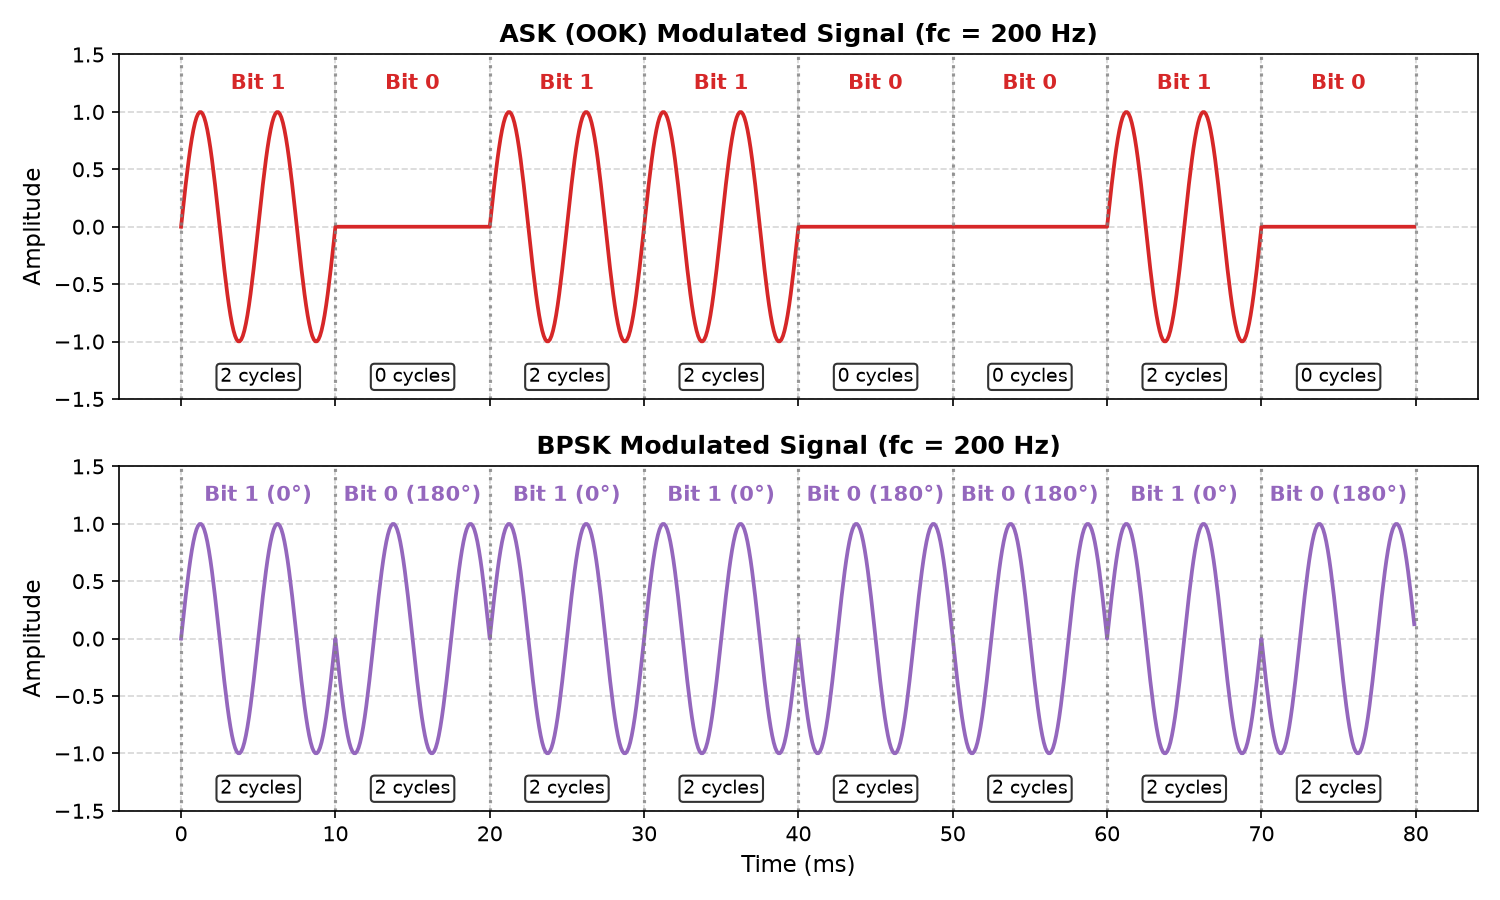
\includegraphics[width=0.88\textwidth]{figures/modulation_plots.png}\\[-1pt]
{\footnotesize\textit{Exact waveform comparison over 80 ms: ASK (carrier on/off) vs. BPSK (constant envelope with $180^\circ$ phase inversion for bit 0).}}
\end{center}

\vspace{-4pt}

\noindent\textbf{\color{themeblue}Receiver Architecture \& Performance Comparison (ASK vs. BPSK):}
\begin{itemize}[leftmargin=12pt, itemsep=1.5pt, topsep=1pt]
    \item \textbf{ASK Demodulation (Envelope Detection):} The received waveform is rectified and low-pass filtered to extract the envelope, followed by a decision threshold $\theta \approx A/2$. Highly vulnerable to noise at low SNR because additive Gaussian noise easily spikes above threshold during bit 0 intervals.
    \item \textbf{BPSK Demodulation (Coherent Correlation):} The received signal is multiplied by an exact, synchronized local carrier replica $c(t) = \cos(2\pi f_c t)$ and integrated over the bit duration $T_b$. Decisions are made against a zero threshold ($\theta = 0\text{V}$), rejecting orthogonal noise.
    \item \textbf{Carrier Frequency Offset Vulnerability (*Lab 03*):} Coherent BPSK requires exact local oscillator frequency synchronization. A frequency offset $\Delta f = 50\text{ Hz}$ across bit duration $T_b = 10\text{ ms}$ causes a full $\pi$ phase rotation ($2\pi \Delta f T_b = 2\pi \cdot 50 \cdot 0.01 = \pi$), flipping signs and reducing detection to pure random guessing ($\text{BER} \approx 0.5$).
\end{itemize}

\vspace{1pt}

\begin{tcolorbox}[
    colframe=accentgreen,
    colback=white,
    arc=1.2mm,
    boxrule=0.5pt,
    left=5pt, right=5pt, top=2.5pt, bottom=2.5pt
]
\textbf{Why BPSK Radically Outperforms ASK in Noise (Euclidean Distance Derivation):}
\begin{itemize}[leftmargin=10pt, itemsep=1pt, topsep=1pt]
    \item \textbf{Constellation Geometry:}
    \begin{itemize}[leftmargin=8pt, itemsep=0.5pt]
        \item In ASK: Symbols are $\{0, A\} \implies d_{\min, \text{ASK}} = A$. Noise margin $= A/2$.
        \item In BPSK: Symbols are $\{-A, +A\} \implies d_{\min, \text{BPSK}} = 2A$. Noise margin $= A$.
    \end{itemize}
    \item \textbf{Noise Immunity:} BPSK provides \textbf{twice the Euclidean distance} ($2A$ vs $A$) for the same peak amplitude. Because error probability decays exponentially with $d_{\min}^2$ ($P_e \approx Q\left(\frac{d_{\min}}{2\sigma}\right)$), BPSK requires $\sim 3\text{ dB}$ to $4\text{ dB}$ less SNR to achieve the same Bit Error Rate.
    \item \textbf{Bit Error Rate (BER) Metric:} $\text{BER} = \frac{\text{Number of Bits in Error}}{\text{Total Transmitted Bits}}$.
    In the midterm test ($\text{SNR} = 7.78\text{ dB}$), ASK yielded $\frac{4}{20} = 0.20$ ($20\%$), while BPSK yielded $\frac{0}{20} = 0.00$ ($0\%$).
\end{itemize}
\end{tcolorbox}

\vspace{2pt}

\clearpage
% =========================================================================
% MODULE 5: CONSTELLATIONS & MULTIPLE ACCESS (CH03 & CH05)
% =========================================================================
\noindent{\Large\bfseries\color{themeblue} 5. Constellation Geometries, Multiple Access \& Error Control}\par\vspace{2pt}

\begin{minipage}[t]{0.46\textwidth}
    \centering
    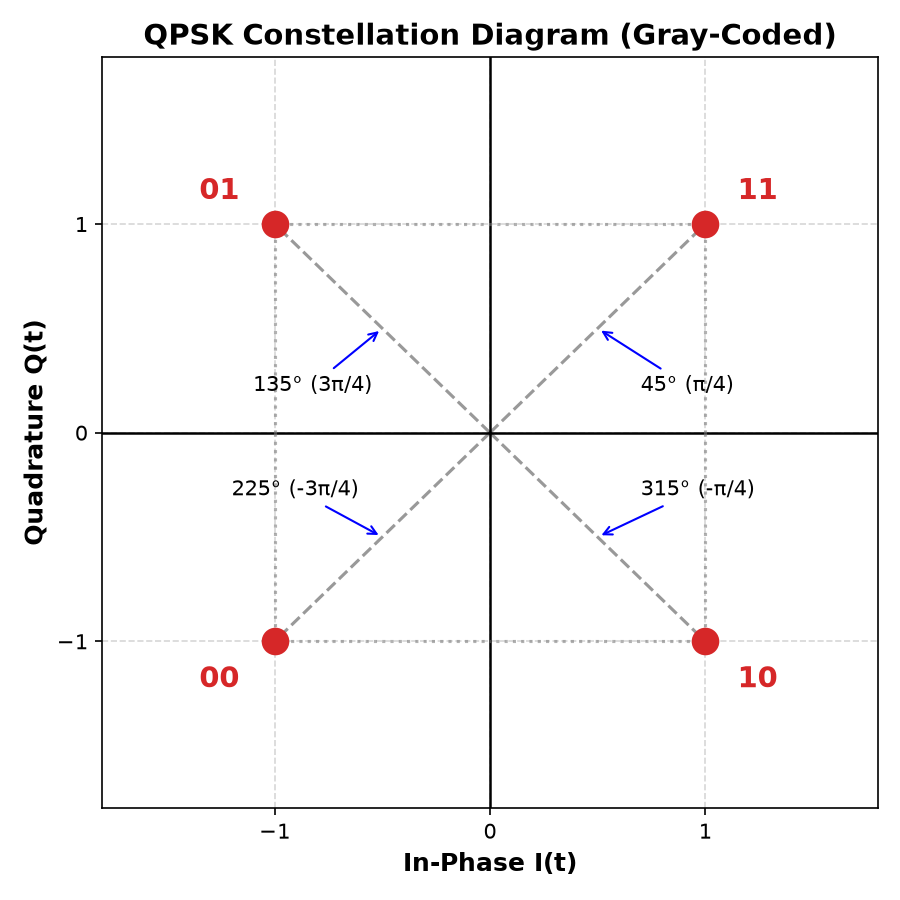
\includegraphics[width=0.62\textwidth]{figures/qpsk_constellation.png}\\[-2pt]
    {\footnotesize\textit{QPSK Gray-Coded Constellation ($I/Q$ orthogonal axes).}}
\end{minipage}
\hfill
\begin{minipage}[t]{0.52\textwidth}
    \footnotesize
    \textbf{QPSK Constellation Mapping (*CH05, Slide 5-21*):}
    \begin{itemize}[leftmargin=10pt, itemsep=1pt]
        \item Quadrant I ($+1, +1$, phase $+45^\circ$): Symbol \textbf{11}
        \item Quadrant II ($-1, +1$, phase $+135^\circ$): Symbol \textbf{01}
        \item Quadrant III ($-1, -1$, phase $-135^\circ$): Symbol \textbf{00}
        \item Quadrant IV ($+1, -1$, phase $-45^\circ$): Symbol \textbf{10}
    \end{itemize}
    \textbf{Gray Coding Advantage:} Adjacent symbols differ by only \textbf{1 bit}. If noise pushes a received point across a boundary into an adjacent quadrant, only a single bit error occurs rather than two.
    
    \vspace{2pt}
    \textbf{16-QAM vs. QPSK Trade-Off (*Part 2, Q5*):}
    16-QAM transmits 4 bits/symbol ($2\times$ throughput of QPSK for same bandwidth). However, 16 constellation points are packed into the same constellation space, making $d_{\min}$ much smaller. Hence, 16-QAM is far more sensitive to noise.
\end{minipage}

\vspace{2pt}

\begin{tcolorbox}[
    colframe=themeblue,
    colback=lightbg,
    arc=1.2mm,
    boxrule=0.5pt,
    left=5pt, right=5pt, top=2.5pt, bottom=2.5pt
]
\footnotesize
\textbf{Multiple Access Taxonomy (*CH03, CH04*):}
\begin{itemize}[leftmargin=12pt, itemsep=1pt]
    \item \textbf{FDMA:} Channel spectrum is sliced into distinct \textbf{frequency bands} allocated continuously to users.
    \item \textbf{TDMA:} Entire bandwidth is shared by assigning distinct \textbf{time slots} to users (*Part 1, Q4*).
    \item \textbf{CDMA:} All users transmit simultaneously across full bandwidth using unique orthogonal \textbf{pseudo-random codes}.
\end{itemize}
\textbf{Error Detection vs. Error Correction (*CH03, CH04, Lab 04*):}
\begin{itemize}[leftmargin=12pt, itemsep=1pt]
    \item \textbf{Parity Bit:} Appends 1 bit to make total 1s even. Detects any odd number of errors ($1, 3, 5$), but fails completely if an \textbf{even number of errors} occurs (2 bit flips leave parity unchanged).
    \item \textbf{ARQ (Automatic Repeat reQuest):} Detects errors (via CRC) and requests retransmission over a feedback channel.
    \item \textbf{Forward Error Correction (FEC):} Transmits structured mathematical redundancy, allowing the receiver to \textbf{detect and correct errors autonomously without retransmission} (*Part 1, Q15*). Crucial for one-way links and real-time streaming.
\end{itemize}
\end{tcolorbox}

\vspace{2pt}

% =========================================================================
% MODULE 6: EXAM RAPID FORMULA CHEAT SHEET & TRAPS
% =========================================================================
\noindent{\Large\bfseries\color{themeblue} 6. Quick Formula Reference \& Common Midterm Traps}\par\vspace{2pt}

\begin{center}
\small
\begin{tabular}{p{4.2cm} p{5.5cm} p{6.2cm}}
\toprule
\rowcolor{lightbg}
\textbf{Concept / Metric} & \textbf{Formula} & \textbf{Exam Trap / Watch Out For} \\
\midrule
\textbf{Shannon Capacity} & $C = B \log_2(1 + \text{SNR})$ & SNR must be in \textbf{linear ratio}, NOT dB! Convert $\text{SNR} = 10^{\frac{\text{SNR}_{\text{dB}}}{10}}$ first. \\
\textbf{Linear SNR to dB} & $\text{SNR}_{\text{dB}} = 10 \log_{10}(P_s / P_n)$ & Power ratio uses $10\log_{10}$, voltage ratio uses $20\log_{10}$. \\
\textbf{Moving Average 1st Null} & $f_{\text{null}} = \frac{f_s}{M}$ & Null is inversely proportional to $M$. Larger $M$ means narrower filter! \\
\textbf{Carrier Cycles per Bit} & $N_{\text{cycles}} = f_c \times T_b = \frac{f_c}{R_b}$ & Count integer cycles carefully per bit window on waveform sketches. \\
\textbf{Path Loss Dependency} & $L \propto f^2 d^2$ & Path loss increases with both distance and frequency (NOT decreases). \\
\textbf{Coherence Time ($T_c$)} & $T_c \gg T_b \implies$ Slow Fading & Car in city $\implies$ high velocity $\implies$ small $T_c \implies$ \textbf{Fast Fading}! \\
\textbf{Coherence Bandwidth ($B_c$)} & $B_c \ll B_s \implies$ Frequency Selective & City buildings $\implies$ large delay spread $\implies$ \textbf{Frequency Selective}! \\
\textbf{Antenna Gain Impact} & $P_r \propto G_t G_r$ & Directional antennas increase received power, reducing path loss impact. \\
\bottomrule
\end{tabular}
\end{center}

\end{document}
